\documentclass[border=1pt]{standalone}
% Shared preamble for the PixelRoot figures: Times text and math to match
% IEEEtran; every figure is drawn at its printed size (no scaling in the paper).
\usepackage[T1]{fontenc}
\usepackage{mathptmx}
\usepackage{amsmath}
\usepackage{xcolor}
\usepackage{tikz}
\usetikzlibrary{arrows.meta,positioning,calc,fit,backgrounds,decorations.pathreplacing,shapes.geometric}
\definecolor{ink}{HTML}{1B2838}
\definecolor{acc}{HTML}{1F5FBF}
\definecolor{grn}{HTML}{1E7B3A}
\definecolor{red}{HTML}{B3261E}
\definecolor{amb}{HTML}{9A6B00}
\definecolor{cu}{HTML}{B87333}
\tikzset{
  >={Stealth[length=1.6mm,width=1.2mm]},
  every picture/.style={line width=0.6pt, font=\footnotesize, color=ink},
  blk/.style={draw=ink, rounded corners=1.5pt, align=center, inner sep=2.5pt,
    minimum height=9mm, fill=white},
  note/.style={font=\scriptsize, align=left, text=ink!80},
}

\begin{document}
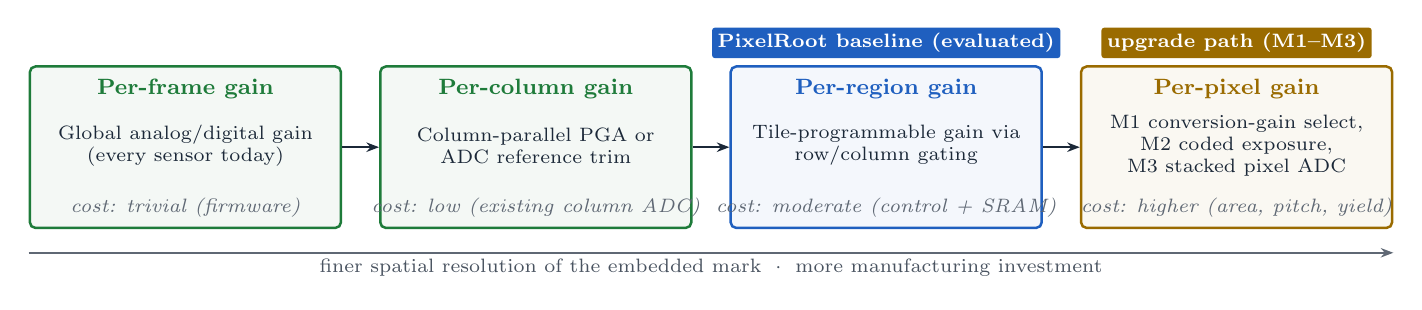
\begin{tikzpicture}
\tikzset{stg/.style={draw=#1, line width=0.9pt, rounded corners=2pt, fill=#1!5,
  minimum width=3.95cm, minimum height=2.05cm, inner sep=0pt}}
\def\dx{4.45}
\foreach \i/\col/\head/\desc/\cost in {
  0/grn/{Per-frame gain}/{Global analog/digital gain\\(every sensor today)}/{trivial (firmware)},
  1/grn/{Per-column gain}/{Column-parallel PGA or\\ADC reference trim}/{low (existing column ADC)},
  2/acc/{Per-region gain}/{Tile-programmable gain via\\row/column gating}/{moderate (control + SRAM)},
  3/amb/{Per-pixel gain}/{M1 conversion-gain select,\\M2 coded exposure,\\M3 stacked pixel ADC}/{higher (area, pitch, yield)}} {
  \node[stg=\col] (s\i) at (\i*\dx,0) {};
  \node[anchor=north, font=\footnotesize\bfseries, text=\col, inner sep=0pt] at ($(s\i.north)+(0,-0.16)$) {\head};
  \node[anchor=center, font=\scriptsize, align=center, inner sep=0pt] at ($(s\i.center)+(0,0.02)$) {\desc};
  \node[anchor=south, font=\scriptsize\itshape, text=ink!70, inner sep=0pt] at ($(s\i.south)+(0,0.14)$) {cost: \cost};
}
\foreach \i [evaluate=\i as \j using int(\i+1)] in {0,1,2} \draw[->, line width=0.8pt] (s\i.east) -- (s\j.west);
% PixelRoot marker
\node[fill=acc, text=white, font=\scriptsize\bfseries, rounded corners=1pt, inner sep=2pt, anchor=south]
  at ($(s2.north)+(0,0.08)$) {PixelRoot baseline (evaluated)};
\node[fill=amb, text=white, font=\scriptsize\bfseries, rounded corners=1pt, inner sep=2pt, anchor=south]
  at ($(s3.north)+(0,0.08)$) {upgrade path (M1--M3)};
% axes
\draw[->, line width=0.7pt, ink!70] ($(s0.south west)+(0,-0.3)$) -- ($(s3.south east)+(0,-0.3)$)
  node[pos=0.5, below, font=\scriptsize, text=ink!80, inner sep=2pt]
  {finer spatial resolution of the embedded mark $\;\cdot\;$ more manufacturing investment};
\end{tikzpicture}
\end{document}
